\section{Arquitetura}

A arquitetura as ser considerada é baseada em \cite{felixnavarro}.
A \textit{RoboCup Small Size League} (SSL) envolve problemas de diversas áreas
da engenharia. Logo, como o objetivo de facilitar compreensão do
problema, a arquitetura a ser considerada é apresentada na figura
\ref{arquitetura_ssl}. Essa arquitetura é composta pelos seguintes
sistemas:

\begin{itemize}
  \item Cameras Visão: Conjunto de câmeras firewire que captura as imagens do
        campo e as envia para a SSL-Vision
  \item Comunicação: Módulo responsável por receber os parâmetros
        dos motores e enviar o comando via onddas de radio para os
        robôs
  \item Execução: Módulo responsável por realizar a tomada de decisões
        em baixo nível de quais ações os robôs devem realizar a partir
        da decisão tomada pelo módulo de Inteligência
  \item Inteligência: Módulo responsável por realizar a tomada de
        decisão em alto nível de quais ações os robôs devem realizar 
        tendo auxílio de um módulo de Simulação
  \item Mundo Real: Mundo real, onde os agentes agem
  \item Referee-Box: \textit{Software} padronizado pela Robocup para que as
        regras da competição sejam cumpridas sem que haja intervenção
        humana excessiva durante uma partida
  \item Simulação: Módulo do software do time responsável por simular
        o ambiente da partida, tendo como entrada os parâmetros do mundo
        real
  \item Software Time 1/2: \textit{Software} do time 1/2
  \item SSL-Vision: \textit{Software} padronizado pela Robocup que permite a
        integração com uma conjunto de câmeras \textit{firewire} que capturam 
        imagens do campo e as processa, extraindo informações sobre os objetos na
        imagem
  \item Time 1/2: Time de robôs que executa os comandos recebidos pelo
        sistema de transmissão do time 1/2
  \item Transmissão 1/2: sistema de transmissão do time 1/2
  \item World Model: Módulo responsável por modelar o mundo e dar
        confiabilidade aos dados que serão enviados ao módulo de
        Inteligência e são oriundos do Referee-Box e SSL-Vision
\end{itemize}

\begin{landscape}
  \begin{figure}[thpb]
    \centering
    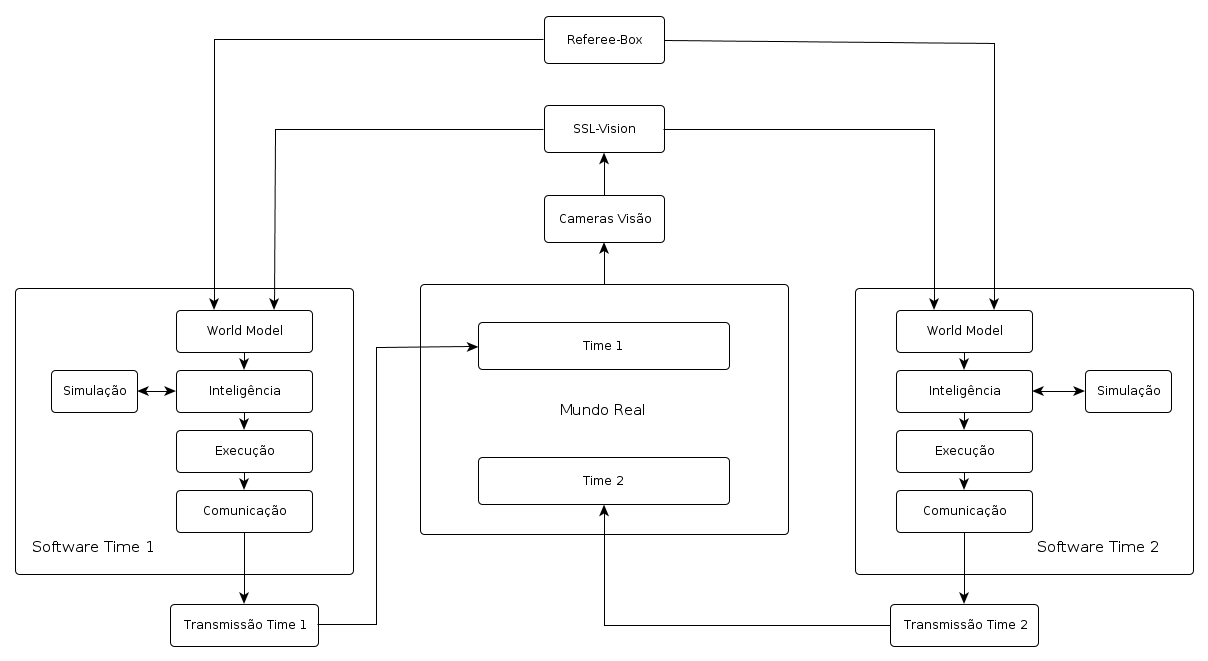
\includegraphics[width=20cm]{imgs/arquitetura_ssl}
    \caption{Arquitetura básica da SSL}
    \label{arquitetura_ssl}
  \end{figure}
\end{landscape}

Apesar de modelar a maioria dos sistemas atualmente empreganos atualmente na
SSL, existem alguns problemas na arquitetura descrita anteriormente. Entretanto,
são necessárias algumas definições apresentadas nas próximas secções para que eles possam ser discutidos.